\documentclass[t 9pt]{beamer}
\title{Long Time Logging}
\subtitle{}
\author{Adrian Dumitrescu}
\institute{ThermoFisher Scientific}
\date{\today}

\begin{document}
    \begin{frame}
        \titlepage
    \end{frame}

    \begin{frame}
        \frametitle{Outline}
        \tableofcontents
    \end{frame}

    \section{Round Robin Database}

    \begin{frame}[t]{Round Robin Database}
        \begin{itemize}
            \item Collects data from multiple data sources
            \begin{itemize}
                \item each data source defines a specific data sample frequency (rate) e.g. RPM value once per second, temperature once every 5 seconds
            \end{itemize}
            \item Stores collected data in multiple archives
            \begin{itemize}
                \item archives are defined at database level
                \item each archive defines a data sample frequency (rate) e.g. one value every second, every minute, every hour
            \end{itemize}
        \end{itemize}
        \begin{figure}
            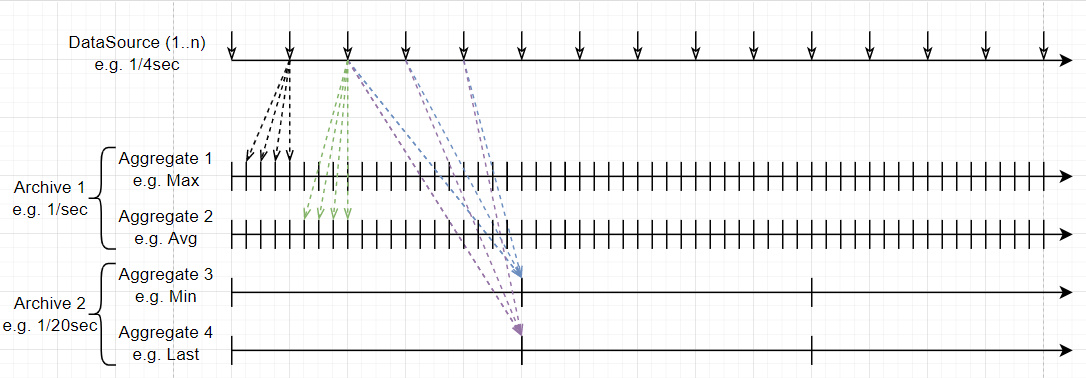
\includegraphics[scale=0.35]{rrdb-structure.jpg}
        \end{figure}
    \end{frame}

    \begin{frame}[t]{Round Robin Database}
        \begin{figure}
            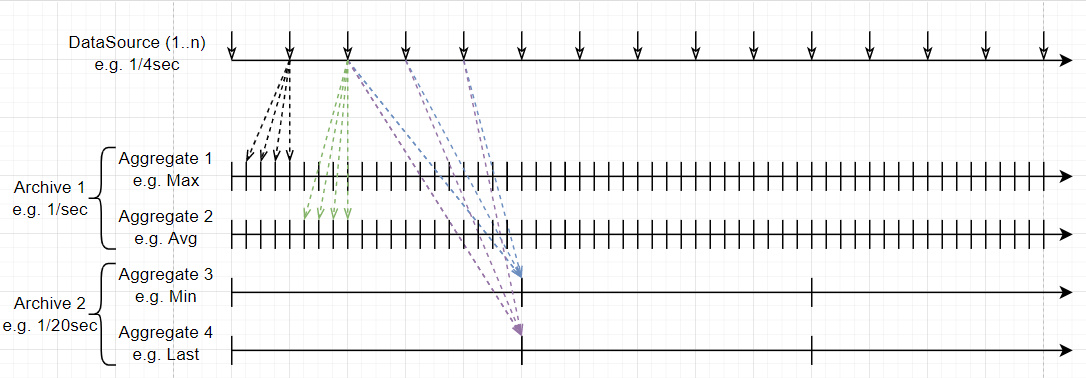
\includegraphics[scale=0.35]{rrdb-structure.jpg}
        \end{figure}
        \begin{itemize}
            \item mismatch between the data sample frequencies of each data source and of each archive
            \item resampling needed before storing: aggregation
            \item each data source defines 0 or more aggregations (from Min, Max, Average, Last)
        \end{itemize}
    \end{frame}

    \begin{frame}[t]{Round Robin Database}
        Trivia: the current database is setup with 3 archives containing data samples for
        \begin{itemize}
            \item every second for 72 hours
            \item every minute for 60 days
            \item every hour for about 9.75 years (probably a mistake; intended to be 10 years)
        \end{itemize}
    \end{frame}

    \section{Data Aggregation}

    \begin{frame}[t]{Data Aggregation}
    \end{frame}


    \section{Section 1}
    \subsection{sub a}

    \begin{frame}
        \frametitle{TAD Accessors}
        Some of the accessors are "tagged" as TAD
        \begin{figure}
            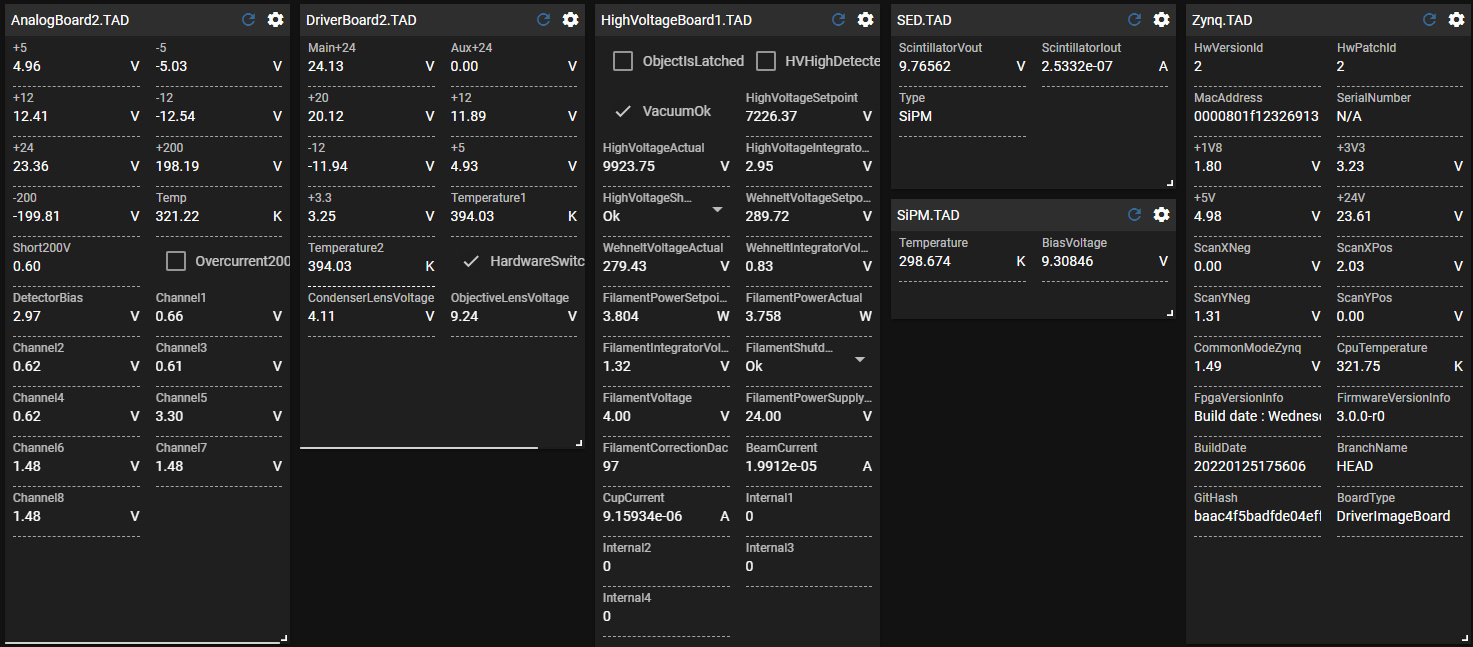
\includegraphics[scale=0.26]{tad-accessors-xl2.jpg}
        \end{figure}
    \end{frame}

    \begin{frame}
        \frametitle{TAD Accessors}
        Accessors "tagged" TAD are also displayed in the Service Tool grouped under TAD
        \begin{figure}
            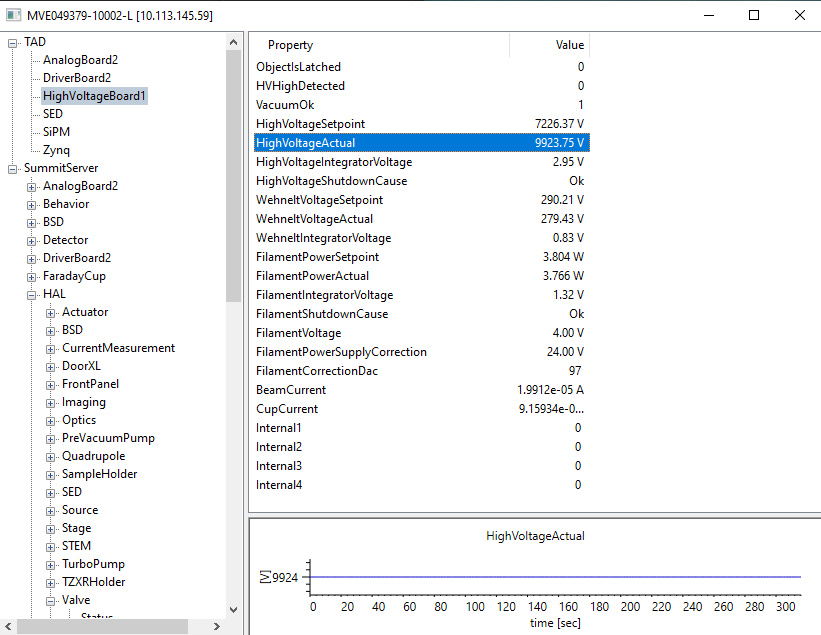
\includegraphics[scale=0.4]{tad-accessors-service-tool.jpg}
        \end{figure}
    \end{frame}

    \begin{frame}
        \frametitle{List (itemize)}
        \begin{itemize}
            \item Point A
            \item Point B
            \begin{itemize}
                \item part 1
                \item part 2
            \end{itemize}
            \item Point C
            \item Point D
        \end{itemize}
    \end{frame}

    \begin{frame}
        \frametitle{List (enumerate)}
        \begin{enumerate}
            \item Point A
            \item Point B
            \begin{enumerate}
                \item part 1
                \item part 2
            \end{enumerate}
            \item Point C
            \item Point D
        \end{enumerate}
    \end{frame}

    \begin{frame}
        \frametitle{Columns}
        \begin{columns}
        \column{0.5\textwidth}
        Lorem ipsum dolor sit amet, consectetur adipiscing elit. Proin in enim feugiat, sodales metus sit amet, ultricies ante. Pellentesque habitant morbi tristique senectus et netus et malesuada fames ac turpis egestas. Ut odio arcu, auctor et massa ut, condimentum ultricies est. Nunc blandit dolor lacus, ac finibus enim ornare at. Vestibulum pretium aliquam tortor, ac molestie nisl vestibulum eget. Sed suscipit leo quis lectus finibus malesuada quis vel arcu. Nunc sagittis diam ac finibus volutpat. In suscipit ac ex interdum gravida.
        \column{0.5\textwidth}
        Lorem ipsum dolor sit amet, consectetur adipiscing elit.
        \begin{figure}
            
\includegraphics[scale=0.5]{caution.pdf}
            \caption{caution!!}
            \end{figure}
        \end{columns}
    \end{frame}
\end{document}